\tikzstyle{linha} = [line width=1.05mm, rounded corners=1mm, yellow!60]
\tikzstyle{caixa} = [rectangle, draw=yellow!60, fill=yellow!60, text width=2cm, text centered, minimum height=0.75cm, font=\footnotesize, rounded corners] 
\tikzstyle{caixalarga} = [rectangle, draw=yellow!35, fill=yellow!60, text width=6cm, text centered, minimum height=0.75cm, font=\footnotesize, rounded corners ]
\begin{tikzpicture}[>={Triangle[angle=60:3mm]}]
 % PICTURE
    \node at (0,0) (LabPick) {\includegraphics[width=18cm]{figures/SmartGridLabNarrower.jpg}};
	% TEXTBOXES
	\node at (-7.5,-0.8) (GridEmu) [caixa] {Grid Emulator\\ac \& dc };
	\node at (-1.5,1.5) (ESSTR) [caixa] {Transformer\\$L_t$ and $R_t$};
	%\node at (3.5,-1.8) (ESSGC) [caixalarga] {Power Electronic Converter (PEC)\\ plus $C_{dc}$, $L_r$, $R_r$, and $C_{ac}$};
    \node at (3.5,1.5) (ESSGC) [caixalarga] {Power Electronic Converter (PEC)\\ plus $C_{dc}$, $L_r$, $R_r$, and $C_{ac}$};
	
 % ARROWS
	\draw [->, linha] (GridEmu) -- ++(0,1);
	\draw [->, linha] (ESSGC) -- ++(0,-0.8) -- ++(2.7,0) -- ++(0,-0.4);
	\draw [->, linha] (ESSTR) -- ++(0,0.7) -- ++(9.6,0) -- ++(0,-1.8);
	
	%\node at (10.9,0) (ConvScopePick) {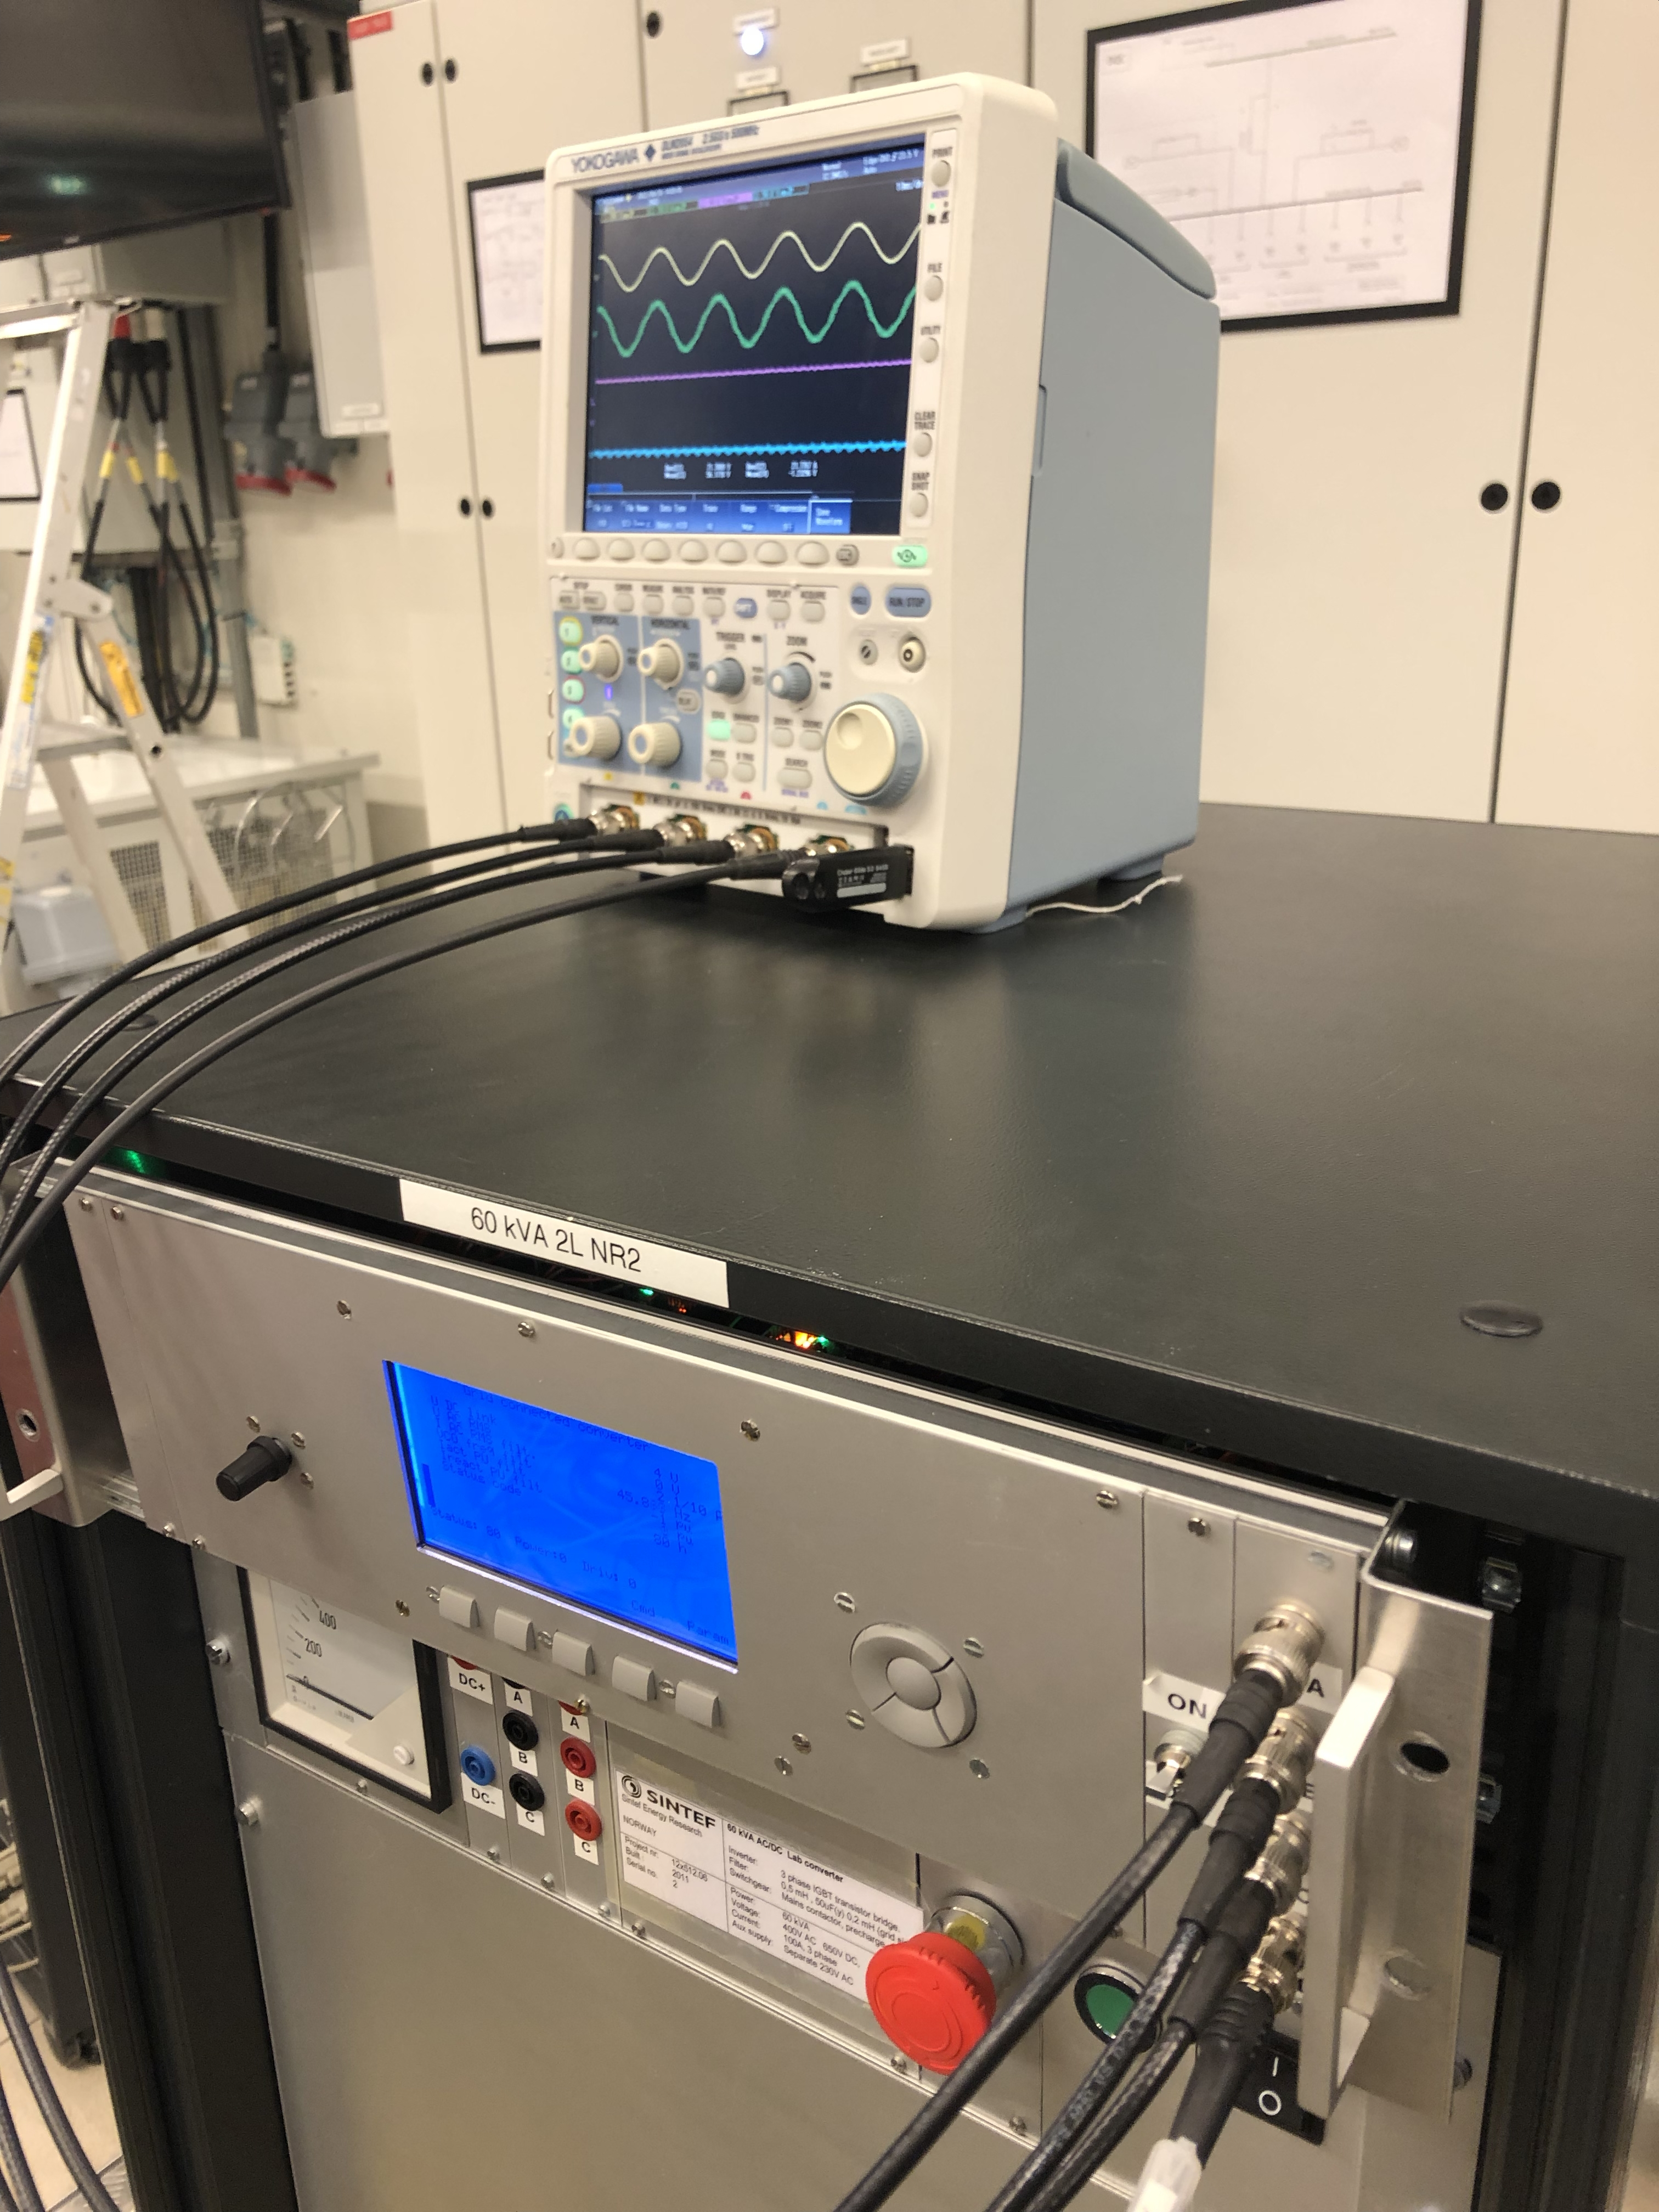
\includegraphics[width=3.6339165cm]{figures/ConverterAndScope.jpg}};
    %\node at (0,-5) (ConvScopePick) {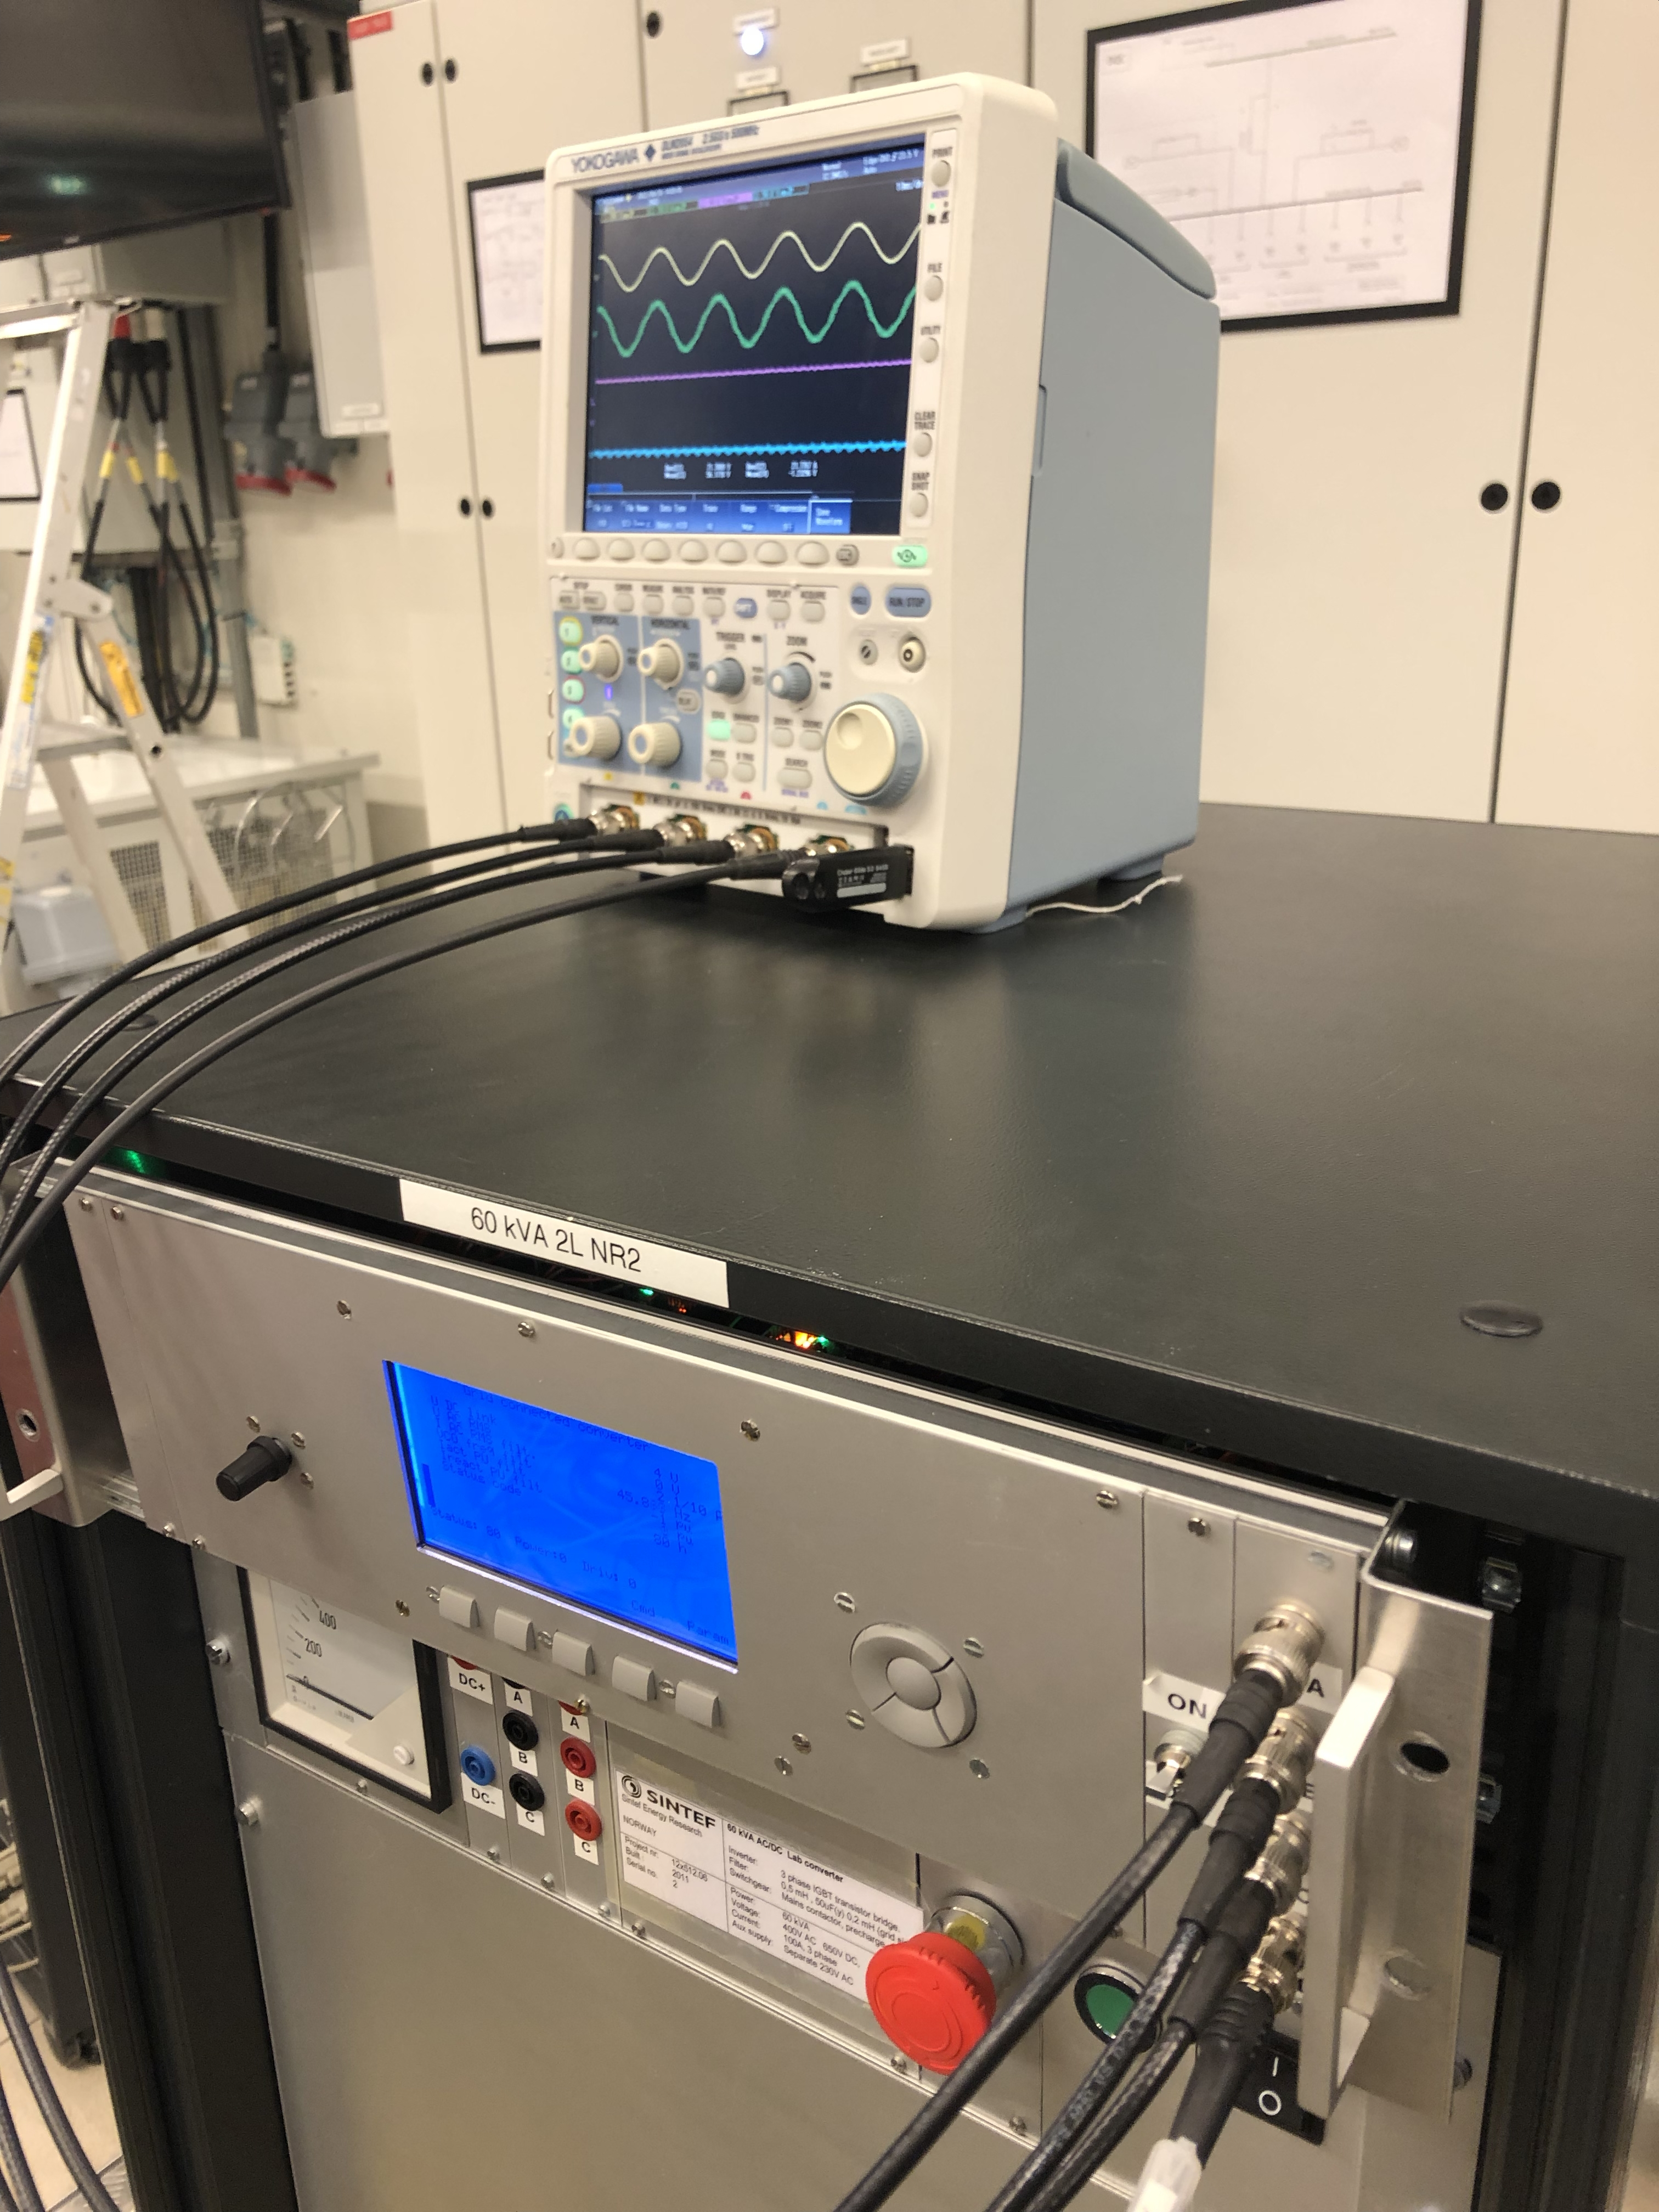
\includegraphics[width=3.6339165cm]{figures/ConverterAndScope.jpg}};
    \node at (0,-5.2) (ConvScopePick) {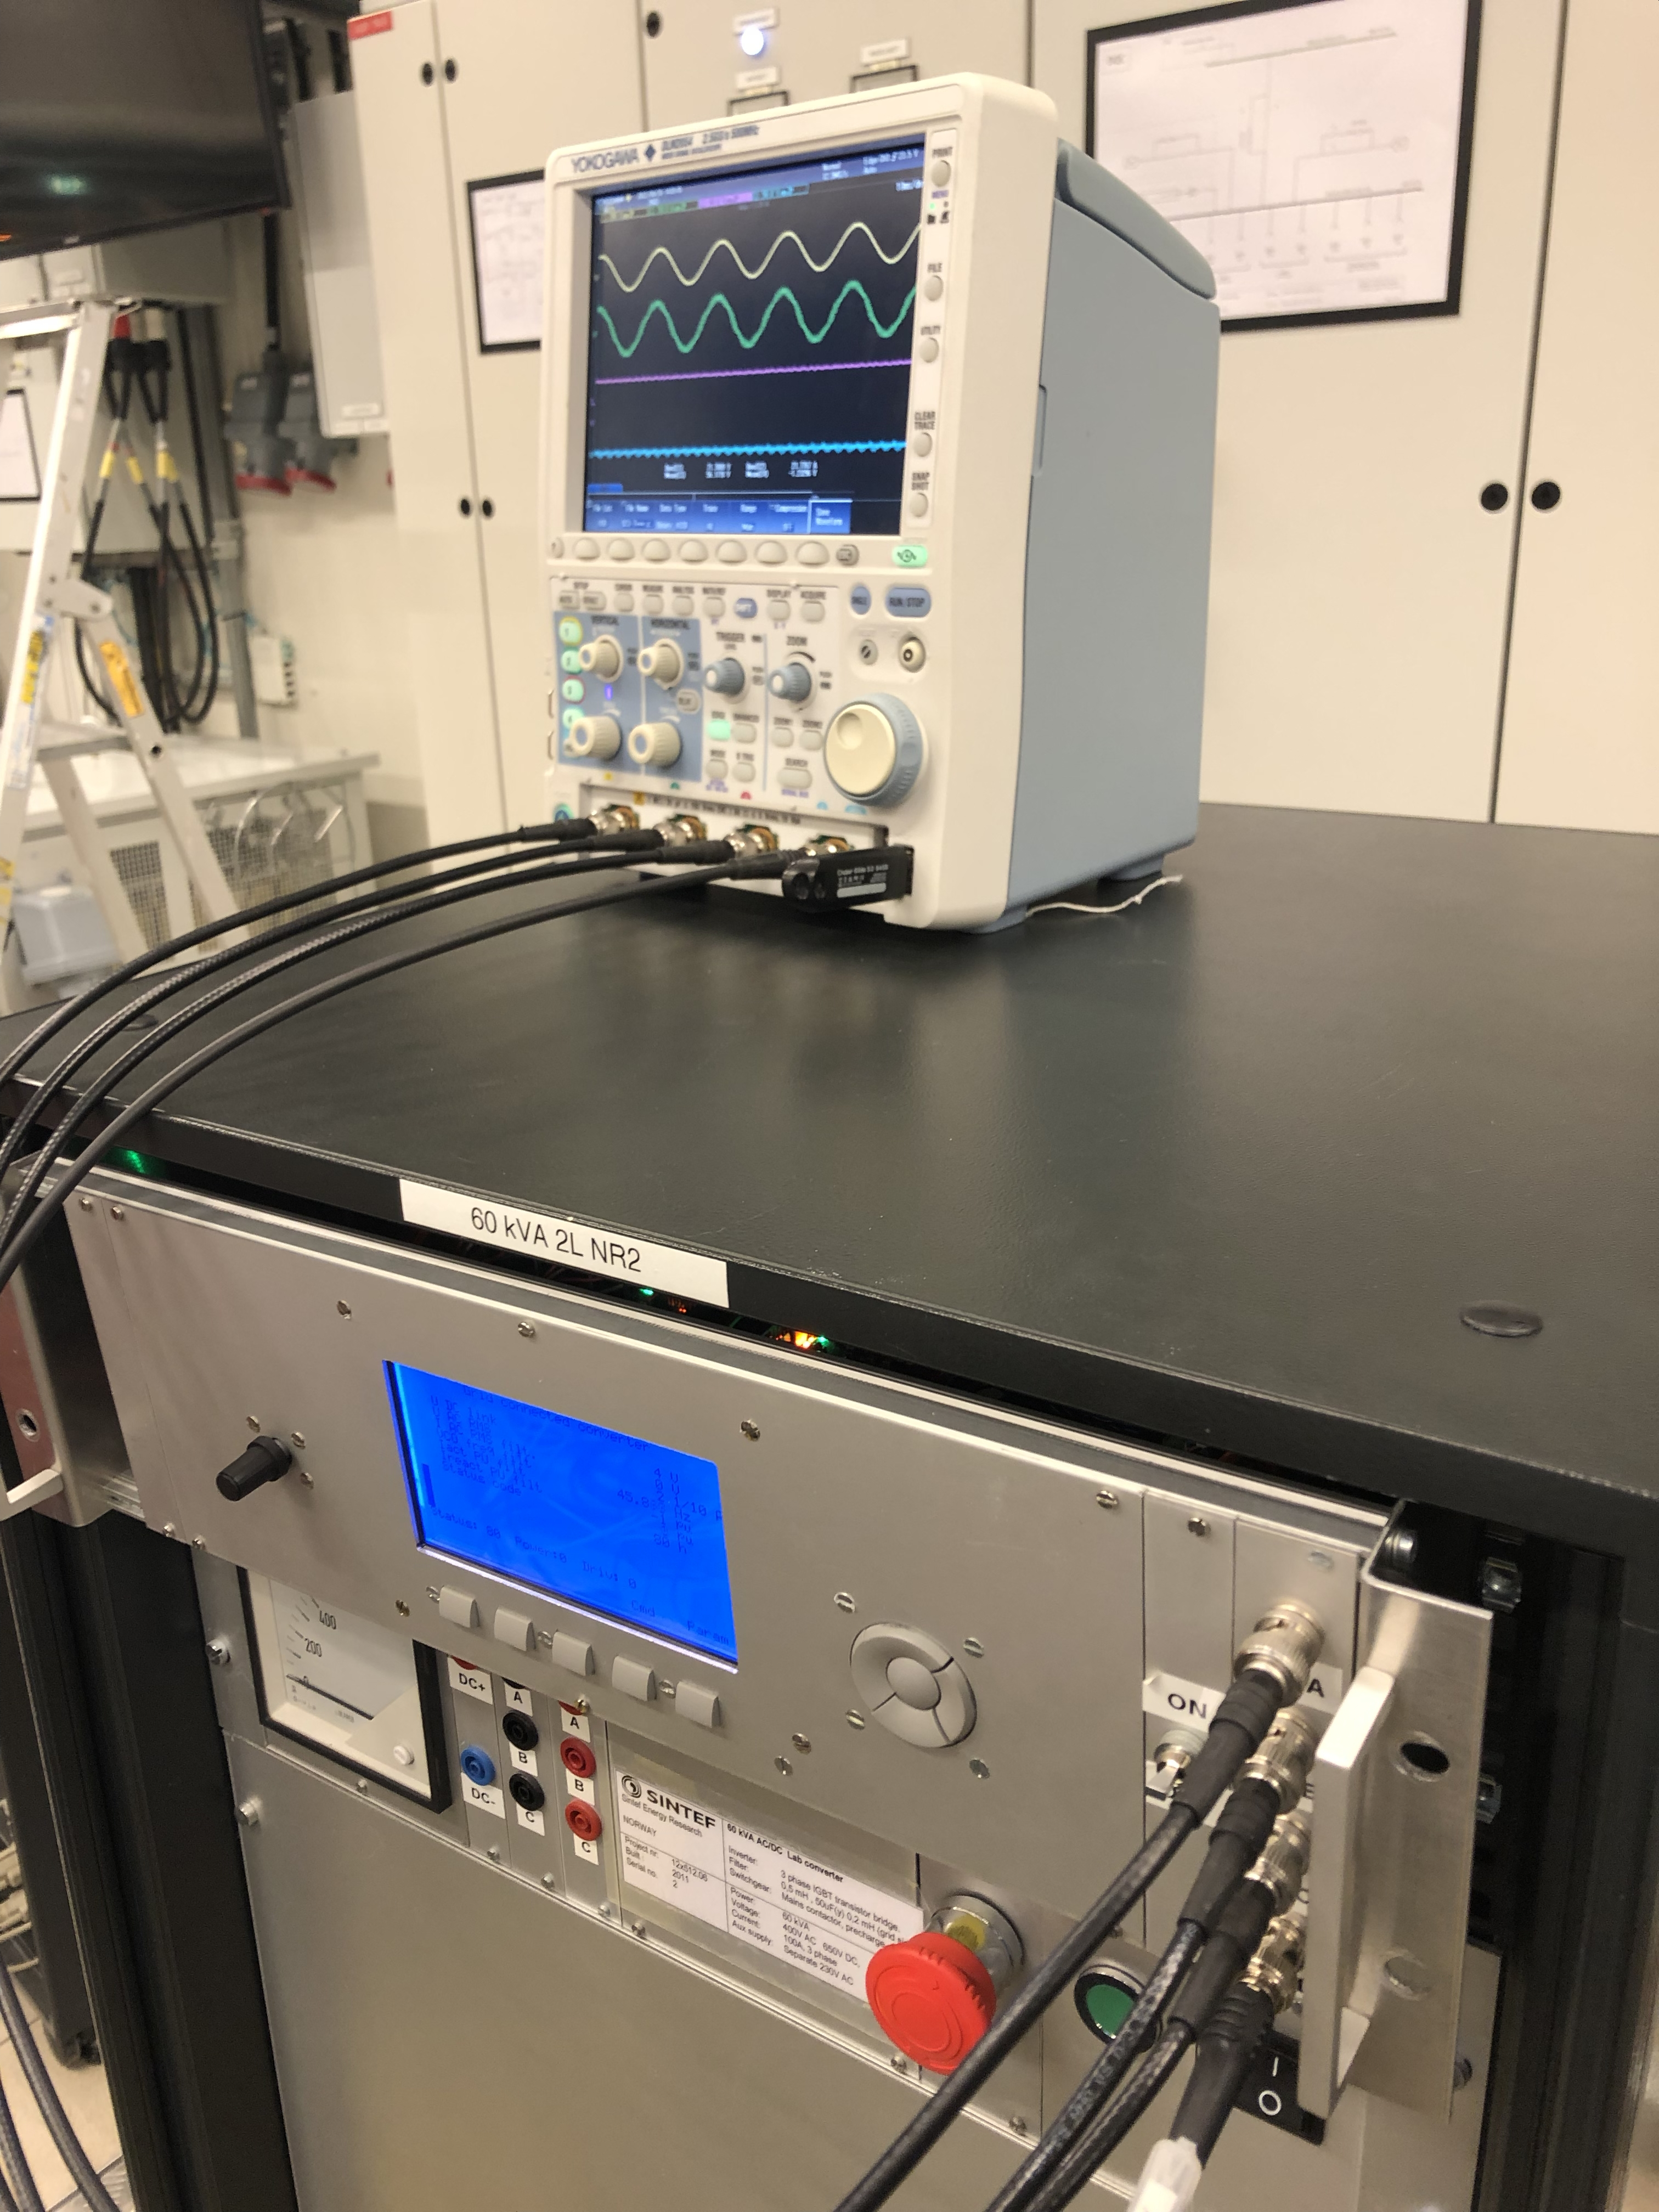
\includegraphics[width=4cm]{figures/ConverterAndScope.jpg}};
	
	\draw [line width=0.25mm, yellow!90] (5.8,0.25) --
	    ++(1,0) --
	    ++(0,-0.7) --
	    ++(-1,0) -- cycle;
	
    %\draw [line width=0.25mm, yellow!90] ($(5.8,0.25)+(1,0)$) -- (9.1, 2.42261104);
	%\draw [line width=0.25mm, yellow!90] ($(5.8,0.25)+(1,-0.7)$) -- (9.1, -2.42261104);

    \draw [line width=0.25mm, yellow!90] ($(5.8,0.25)+(0,0)$) -- (-2, -2.52);
    \draw [line width=0.25mm, yellow!90] ($(5.8,0.25)+(1,-0.7)$) -- (2, -7.87);
 
	\node at (0,-5.5) (ConvScope) [caixa] {PEC with\\ Oscilloscope};
	
\end{tikzpicture}
